\documentclass[10pt,a4paper]{article}
\usepackage[a4paper,margin=1.7cm]{geometry}
\usepackage[T1]{fontenc}
\usepackage[utf8]{inputenc}
\usepackage{lmodern}
\usepackage{microtype}
\usepackage{graphicx}
\usepackage{wrapfig}
\usepackage{booktabs}
\usepackage{tabularx}
\usepackage{array}
\usepackage{enumitem}
\usepackage{titlesec}
\usepackage{xcolor}
\usepackage{xurl}
\usepackage[hidelinks]{hyperref}

% The main figure is made by code/group5_kpis.Rmd and saved as output/fig_main.png
\graphicspath{{../output/}{./}}

\titleformat{\section}{\normalsize\bfseries}{\thesection}{0.6em}{}
\titlespacing*{\section}{0pt}{0.8ex}{0.4ex}
\setlist{nosep,leftmargin=1.2em}
\setlength{\parindent}{0pt}
\setlength{\parskip}{0.45ex}
\newcommand{\lab}[1]{{\footnotesize\textsc{[#1]}}}
\newcolumntype{L}{>{\raggedright\arraybackslash}X}
\definecolor{alert}{HTML}{C0392B}
\newcommand{\red}{\textcolor{alert}{\textbf{red}}}

\begin{document}

\begin{center}
{\large\bfseries What should FZS track every year? Five indicators for illegal gold mining in Peru}\\[0.4ex]
{\small Group 5 (Giant River Turtle): Likitha Yenuga, Laura Pérez, Pietro Maran, Erion Vathi, Santiago Sierra\\
Data for Good, Question 5 \,·\, October 2026 \,·\, Replication files: \url{https://github.com/SantiagoSierraIba/fzs-gold-mining-kpis}}
\end{center}

\section{The question}

The Frankfurt Zoological Society (FZS) works to protect wilderness areas in the Peruvian Amazon, including the Tambopata National Reserve and its surroundings in Madre de Dios. Illegal gold mining is one of the main threats to these areas. FZS reports every year to donors and governments on whether the situation is getting better or worse. The yearly satellite maps of mining area, the main public source, are published 5 to 17 months after the year ends (MapBiomas Peru, 2023--2026). During the 2021--2023 surge (annual additions of 4,940, 10,540 and 19,339~ha), the first of these maps, with data up to 2021, appeared only in March 2023 (Panamericana, 2023).

We ask: \textbf{which small set of numbers should FZS check every year, so that it sees trouble earlier and knows where to act?} We study Madre de Dios, which holds 95\% of the mining area in Peru's Amazon (112,622~ha in 2025), from 2016 to the third quarter of 2026, and test each indicator on the 2021--2023 surge using only what was public at the time. We propose indicators at three speeds: \emph{early} (moves before mining appears on maps), \emph{now} (shows where mining is this quarter) and \emph{late} (slow but trusted, for donor reports). All claims below are descriptions or predictions; we make no causal claims.

\section{Data and provenance}

Every file is in \texttt{data\_raw/} as downloaded and listed in \texttt{DOWNLOAD\_LOG.csv}; the notebook stops if any of its 26 checks against the publisher fails.

\vspace{-0.6ex}
{\small
\begin{tabularx}{\textwidth}{@{}p{5.6cm}Lr@{}}
\toprule
Dataset (publisher, version) & Check: our number = publisher's & Value \\
\midrule
Land cover and transitions by department, buffer zone and protected area (MapBiomas Peru, Collection 4) & Madre de Dios, mining area, 2025 & 112,622 ha \\
Monthly commodity prices (World Bank Pink Sheet, Oct 2026) & Gold price, August 2026 & \$4,411/oz \\
Exchange rate, prices, gold exports and production (BCRP) & Soles per US dollar, Sep 2026 & 3.38 \\
New mining detections and scar map (Amazon Mining Watch, 3 Oct 2026) & Peru, mined area until 2026 Q2 (dashboard: 179.9k ha) & 179,874 ha \\
Protected areas, buffer zones, native communities; mining concessions (SERNANP; INGEMMET); boundaries (GADM 4.1) & Used to place each detection; AMW Tambopata reserve total matches AMW's own table (within 1\%) & --- \\
Published figures (MAAP \#233, \#241) & Typed by hand with report and date & --- \\
\bottomrule
\end{tabularx}}

\section{Findings}

\begin{wrapfigure}[23]{r}{0.56\textwidth}
\vspace{-3.2ex}
\centering
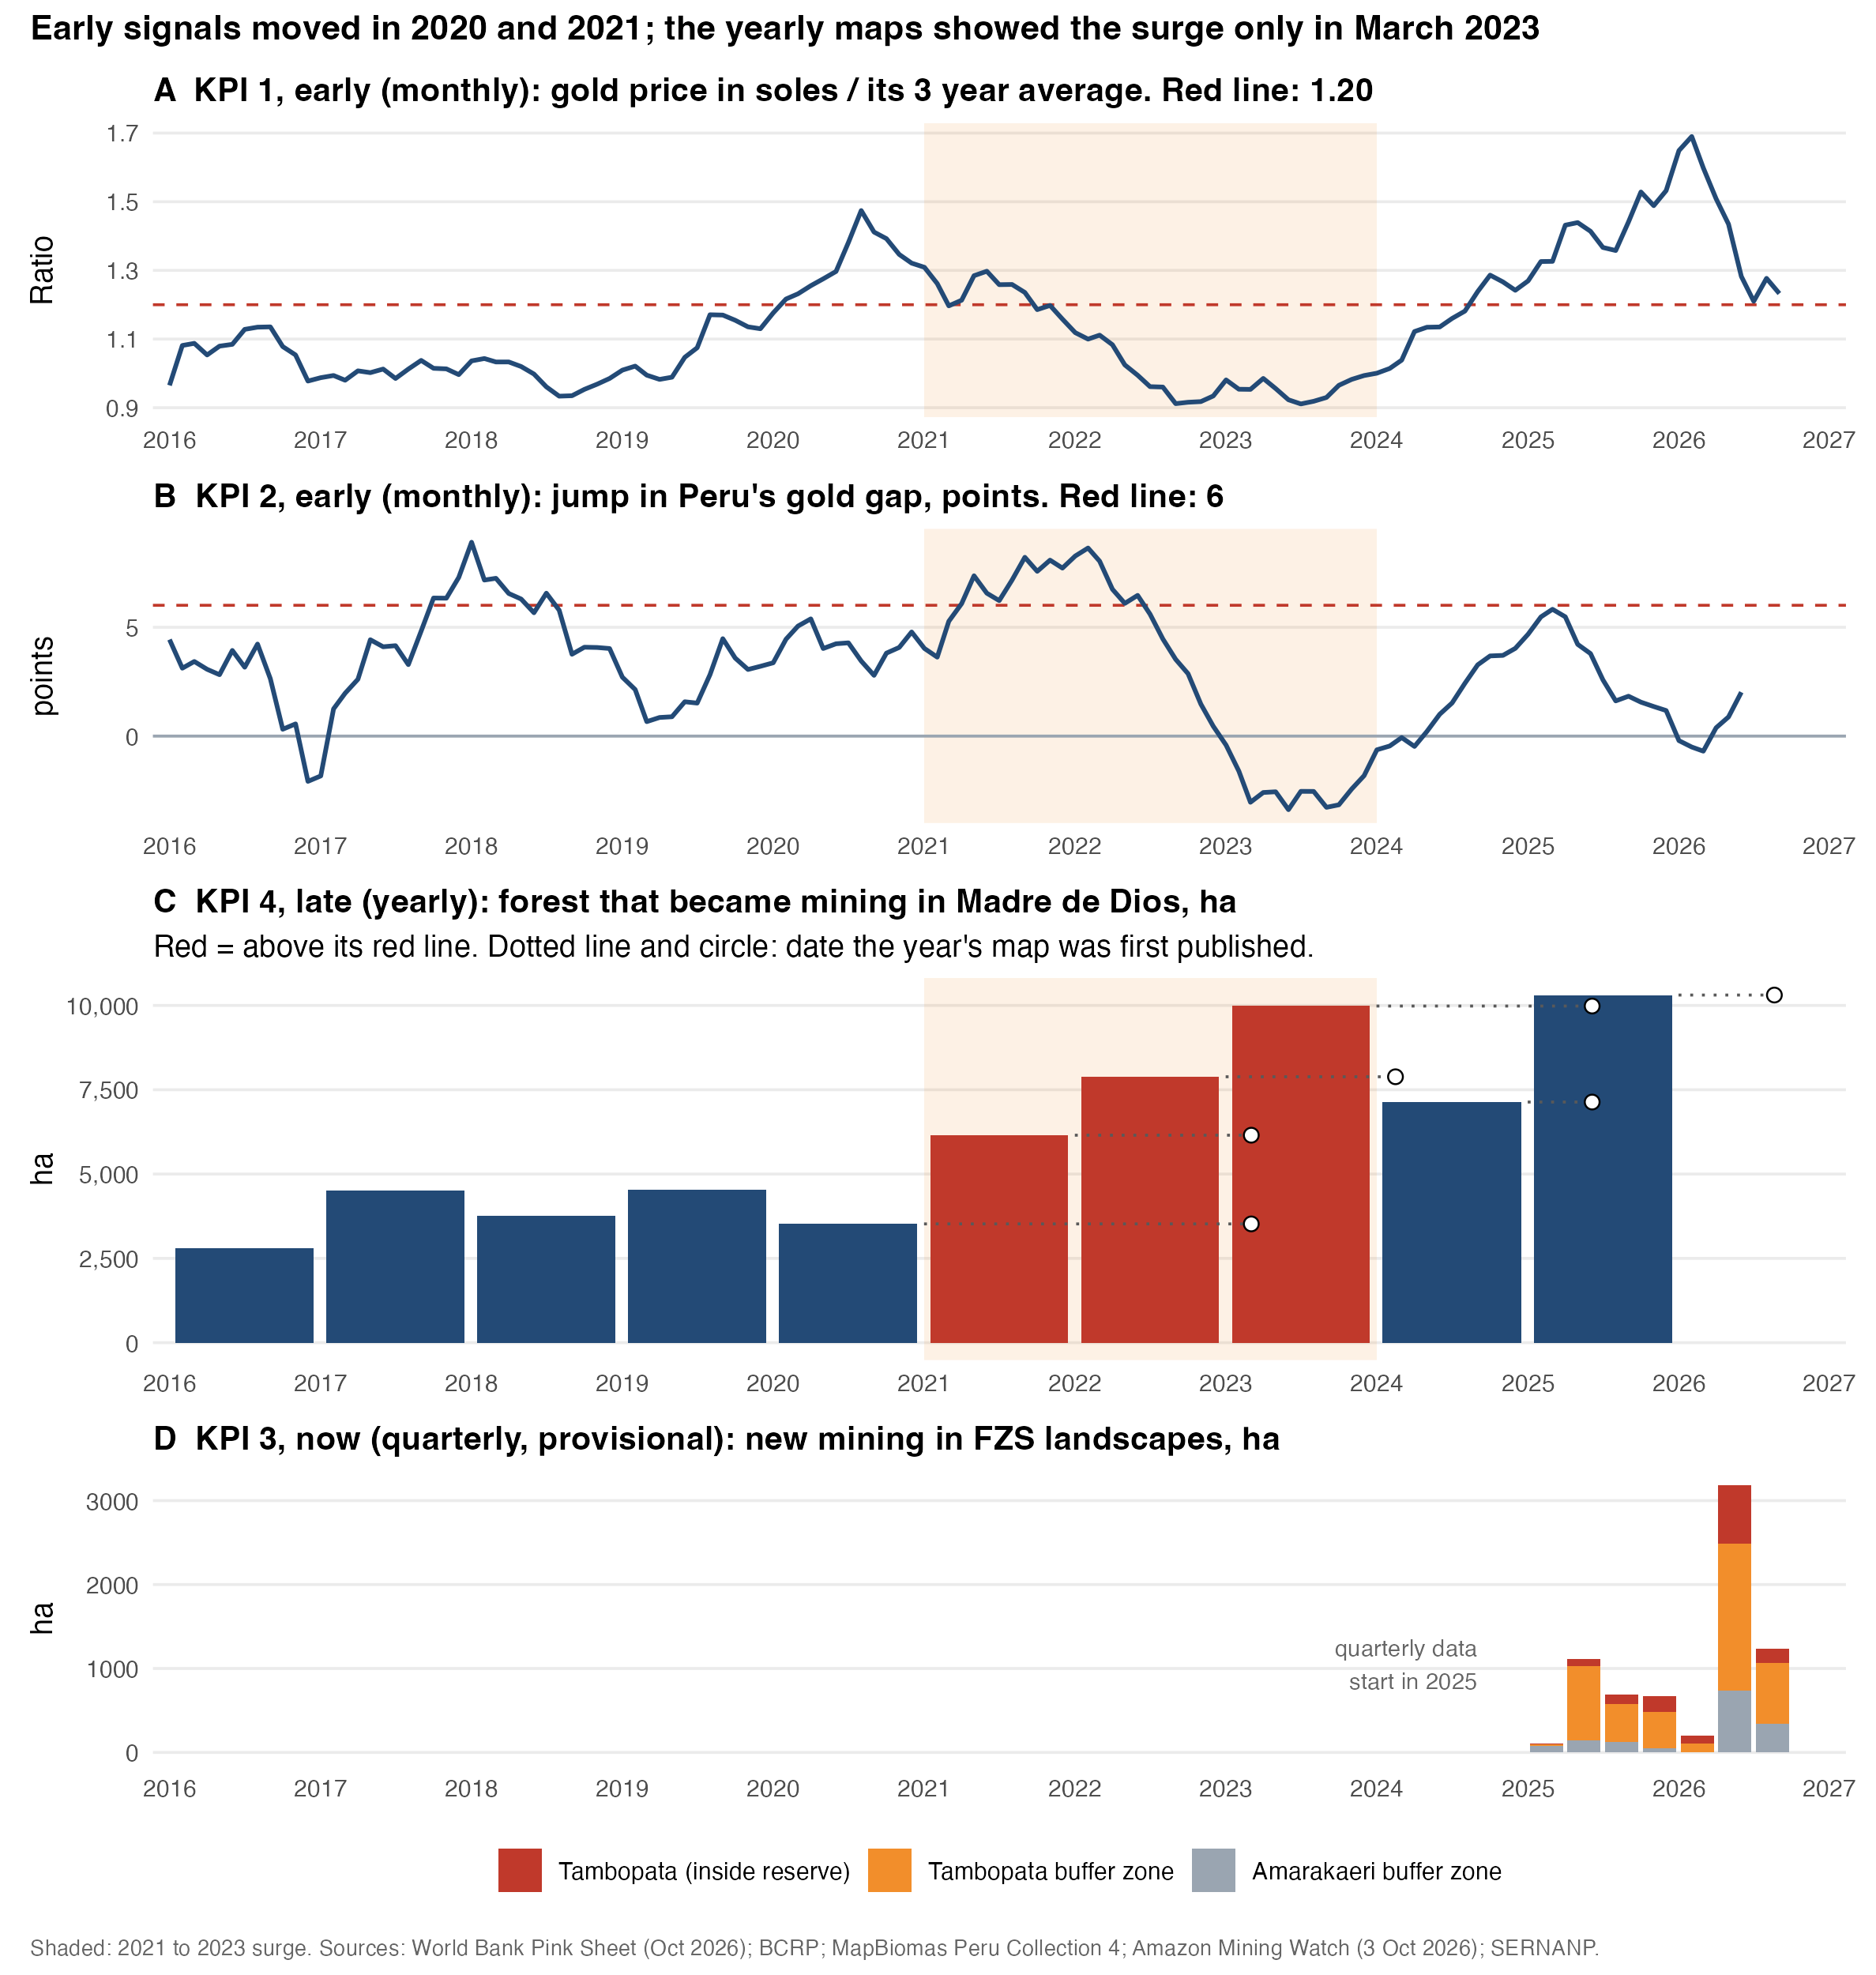
\includegraphics[width=0.56\textwidth]{fig_main.png}
\vspace{-4.5ex}
\end{wrapfigure}

\textbf{Main point.} \lab{Description} The early signals moved in 2020 and 2021; the yearly maps showed the surge only in March 2023 (figure). The gold price in soles rose above its red line in February 2020, public by March 2020. Peru's gold gap jumped in April 2021, public by June 2021. Forest turned into mining in Madre de Dios crossed its red line in 2021, 2022 and 2023, but the 2021 map was published on 3 March 2023. No single indicator is enough: the early ones say \emph{that} pressure is rising, not \emph{where}; the late ones say how much, 5 to 17 months later.

\textbf{Water relabelled as mining.} \lab{Description} The 2023 jump was inflated: 39\% of the land that became ``mining'' that year had been water the year before (9,616~ha). These are likely flooded old pits that the map labelled again: mining ponds are hard to classify from space (Caballero Espejo et al., 2018; Camalan et al., 2022), and the same jump appears in the rest of Peru. So our yearly indicator counts only \emph{forest} that became mining. On that measure 2025 is the record year (10,308~ha).

\textbf{Where mining is now.} \lab{Description} Inside the Tambopata National Reserve, Amazon Mining Watch shows 966~ha of new mining in the first three quarters of 2026, against 194~ha a year earlier (164 detections against 19). MAAP \#241 independently reports more than 400~ha of mining deforestation inside the reserve in 2025. The share of new detections in reserves and buffer zones rose from 16\% in 2021--2023 to 40\% in 2026. \lab{Prediction} If this continues, the 2026 yearly map is likely to show the most forest lost to mining inside the reserve in our data.

\textbf{Comparison.} \lab{Description} Mean yearly additions to the mining area in buffer zones rose from 1,468~ha (2016--2020) to 2,529~ha (2021--2025); in the rest of Madre de Dios from 2,405 to 8,044~ha. We start the second period in 2021, the first year forest turned into mining crossed its red line; the rest of the department faces the same gold price, roads and weather, but it is not a control group. The surge was mostly outside the buffer zones; the move into protected land came after it.

\vspace{0.3ex}
{\footnotesize
\begin{tabularx}{\textwidth}{@{}p{3.3cm}p{1.6cm}p{3.5cm}LL@{}}
\toprule
Indicator (speed, update) & Source & Today & Red when & Action when red \\
\midrule
1 Gold price in soles ÷ its 3-year average (early, monthly, 1 month) & Pink Sheet; BCRP & 1.23 (Sep 2026): \red & Ratio reaches 1.20 & Plan patrols and flights for the next dry season \\
2 Gold gap: exports minus declared production (early, monthly, 2 months) & BCRP & 51\% of exports; +2.0 points: not red & Jump of more than 6 points on a year earlier & Press buyers and ministries for gold traceability \\
3 New mining in FZS landscapes (now, quarterly, days) & AMW; SERNANP & Reserve 966 ha in Q1--Q3 2026: \red & Reserve: a quarter above 56 ha; buffer zones: +25\% on same quarters & Send locations to SERNANP and the prosecutor; overflight \\
4 Forest that became mining (late, yearly, 5--17 months) & MapBiomas Peru & Reserves 175 ha, buffer zones 2,992 ha (2025): \red & Above previous 5-year mean + 2 SD & Report to donors and government, naming the place \\
5 New mining outside Madre de Dios (now, quarterly, days) & AMW; GADM & 2,168 ha in Q1--Q3 2026 ($-$11\%): not red & +25\% on same quarters last year & Alert SERNANP and regional government to a new front \\
\bottomrule
\end{tabularx}}

\section{What FZS can do with this}

\textbf{What FZS can learn.} Three of five indicators are red today, and the clearest signal is inside FZS's own landscape: new mining in the Tambopata reserve is five times last year's, and buffer zones and native communities are up 89--219\%. FZS can act on this now, with the quarterly locations, rather than wait for the 2026 map in 2027. The gold price is high again (1.23), so pressure is likely to continue next dry season \lab{Prediction}.

\textbf{Why it could mislead.} \emph{Selection and hindsight:} we chose the red lines after seeing the surge, so the backtest shows what would have happened, not proof; the gold-gap rule also fired in 2017--2018 with no surge after it. \emph{Omitted variables:} COVID-19, Operation Mercurio (2019) and weaker enforcement happened at the same time as the price rise, so we cannot say the price caused the surge. \emph{Reverse causation:} more mining also raises exports, so the gold gap partly reflects mining rather than predicting it. \emph{Measurement error:} each MapBiomas collection revises the past (Madre de Dios 2022: about 82,900~ha in Collection 2, 74,966~ha in Collection 4, $-$10\%); the newest year is the least corrected; Amazon Mining Watch rebuilt its model in 2026 and its quarterly data are provisional; the 2023 water relabelling may be a method change, since it also appears in the rest of Peru. \emph{What the data cannot see:} dredges on rivers (MAAP \#233, introduction, counts mining in 225 water bodies and 989 dredges in Loreto since 2017), mercury in water, fish and people, and legality, since only mining inside a reserve is clearly illegal.

\textbf{What would let us say more.} Two more years of data, to test the red lines fairly on 2026--2027. Dated archives of each MapBiomas and Amazon Mining Watch version, so FZS reports every number with its version. Ground checks of the quarterly detections inside the reserve. River monitoring (dredge counts, mercury sampling) to cover what land maps miss. To estimate effects rather than describe them, a comparison of similar areas with and without enforcement, before and after it starts.

% ------------------------------------------------------------------
\newpage
\section*{References}
{\small
\begin{itemize}
\item MapBiomas Peru (2026). Collection 4 of land cover and use, statistics: \emph{Límites políticos}, \emph{Zona de amortiguamiento}, \emph{Áreas naturales protegidas} (COVERAGE\_4, TRANSITION\_4). \url{https://peru.mapbiomas.org/descargas/estadisticas/}. Accessed 11--15 Oct 2026.
\item World Bank (2026). Commodity Price Data (Pink Sheet), monthly, updated 2 Oct 2026. \url{https://www.worldbank.org/en/research/commodity-markets}. Accessed Oct 2026.
\item Banco Central de Reserva del Perú (2026). BCRPData series PN01234PM, PN38705PM, PN38792BM, RD12978DM. \url{https://estadisticas.bcrp.gob.pe}. Accessed Oct 2026.
\item Earth Genome and Amazon Conservation (2026). Amazon Mining Watch: \nolinkurl{amazon_basin_detections.geojson}, \nolinkurl{amazon_basin_mining_scar_masks.tif}, README of 3 Oct 2026; dashboard \url{https://amazonminingwatch.org} (Peru, read 15 Oct 2026). \url{https://source.coop/earthgenome/amazon-mining-watch}. CC BY 4.0. Accessed Oct 2026.
\item SERNANP (2026). Protected areas, buffer zones, native communities and INGEMMET mining concessions (download service). \url{https://geoservicios.sernanp.gob.pe}. Accessed Oct 2026.
\item GADM (2022). Version 4.1, Peru level 1. \url{https://gadm.org}. Accessed 11 Oct 2026.
\item MAAP \#233 (29 Sep 2025). Current situation of gold mining in the Peruvian Amazon. Amazon Conservation. Introduction. \url{https://www.maapprogram.org/gold-mining-peru-amazon/}. Accessed 12 Oct 2026.
\item MAAP \#241 (12 May 2026). Illegal mining is once again pushing deeper into one of Peru's most iconic protected areas. Amazon Conservation. \url{https://www.amazonconservation.org/illegal-mining-is-once-again-pushing-deeper-into-one-of-perus-most-iconic-protected-areas/}. Accessed 12 Oct 2026.
\item MapBiomas Peru (5 Feb 2024). Alertan sobre pérdida de glaciares y vegetación natural en Perú (Collection 2, presented 15 Feb 2024; Madre de Dios mining area, 2022). \url{https://peru.mapbiomas.org/2024/02/05/alertan-sobre-perdida-de-glaciares-y-vegetacion-natural-en-peru/}. Accessed 13 Oct 2026.
\item MapBiomas Peru (2025). Colección 3: ``El 5 de junio de 2025 se presentó la Colección 3''. \url{https://old-peru.mapbiomas.org/en/?p=138}. Accessed 16 Oct 2026.
\item Panamericana (3 Mar 2023). En 37 años, Perú perdió 49.9\% de sus glaciares y 3.9\% de su vegetación natural (MapBiomas Peru Collection 1). \url{https://panamericana.pe/nacionales/374521-37-anos-peru-perdio-49-9-glaciares-3-9-vegetacion-natural}. Accessed 13 Oct 2026.
\item Caretas (20 Aug 2026). Perú perdió 3,7 millones de hectáreas de vegetación natural en 41 años (MapBiomas Peru Collection 4). \url{https://caretas.pe/?p=828926}. Accessed 13 Oct 2026.
\item Caballero Espejo, J., Messinger, M., Román-Dañobeytia, F., Ascorra, C., Fernandez, L. E. and Silman, M. (2018). Deforestation and forest degradation due to gold mining in the Peruvian Amazon: a 34-year perspective. \emph{Remote Sensing}, 10, 1903, Section 2 and Figure S1. \url{https://doi.org/10.3390/rs10121903}. Course reading, accessed Oct 2026.
\item Camalan, S., Cui, K., Pauca, V. P., Alqahtani, S., Silman, M., Chan, R., Plemmons, R. J., Dethier, E. N., Fernandez, L. E. and Lutz, D. A. (2022). Change detection of Amazonian alluvial gold mining using deep learning and Sentinel-2 imagery. \emph{Remote Sensing}, 14, 1746, Section 1 and Figure 1. \url{https://doi.org/10.3390/rs14071746}. Course reading, accessed Oct 2026.
\end{itemize}}

\section*{Appendix A: Data log}
{\small The full data log is \texttt{DOWNLOAD\_LOG.csv} in the replication folder: one row per raw file, with publisher, link, download date, settings and the check number. Every number in this brief is in \nolinkurl{output/numbers_in_brief.csv}, produced by \nolinkurl{code/group5_kpis.Rmd}; numbers typed from reports are marked ``typed by hand'' with report and date.}

\section*{Appendix B: AI output used for part 4}
{\small
\textbf{Prompt.} ``Here is my comparison: units are the buffer zones of protected areas in Madre de Dios, Peru, and the rest of the department; the years are 2016--2020 and 2021--2025; the outcome is the mean yearly addition to the area classified as mining (MapBiomas Peru, Collection 4). Buffer zones: 1,468 ha per year, then 2,529. Rest of Madre de Dios: 2,405, then 8,044. List the reasons this comparison could mislead, distinguishing omitted variables, reverse causation, selection of units, and measurement error in the outcome. For each, say what data or design would fix it.''

\textbf{AI answer} (Claude, Anthropic, 15 Oct 2026, unedited):
\begin{itemize}
\item \emph{Omitted variables.} The gold price, COVID-19 job losses and changes in enforcement (Operation Mercurio from 2019) all changed between the two periods and may affect the two areas differently. Fix: add these as controls in a regression with area and year fixed effects, or compare areas that faced the same enforcement.
\item \emph{Reverse causation.} Enforcement and the legal status of land respond to mining: more mining in an area can bring more patrols or new rules. Fix: use timing that was set in advance (dates of operations announced earlier) or an event-study design.
\item \emph{Selection of units.} Buffer zones were drawn around reserves in specific places, not at random; the ``rest'' includes the legal mining corridor, which is meant for mining. Fix: compare with areas that had similar mining before 2016, or split the rest into corridor and non-corridor land.
\item \emph{Measurement error in the outcome.} The mining class includes old pits relabelled from water, legal and illegal mining, and is revised in each collection; the latest year is least corrected. Fix: use forest-to-mining transitions, record the collection, and check against independent sources (MAAP, Amazon Mining Watch).
\end{itemize}
\textbf{Our edited version} is the paragraph ``Why it could mislead'' in part 4: we kept the four categories, added our own evidence for each (the 2017--2018 false alarm, the Collection 2 vs 4 revision, the 2023 water relabelling) and what land-cover data cannot see.}

\end{document}
